\documentclass[11pt]{article}
\usepackage{spikey}
\usepackage{amsmath}
\usepackage{amssymb}
\usepackage{soul}
\usepackage{float}
\usepackage{graphicx}
\usepackage{subfig}
\usepackage{hyperref}
\usepackage{xcolor}
\usepackage{chngcntr}
\usepackage{centernot}
\usepackage{datetime}
\usepackage[shortlabels]{enumitem}

\usepackage[margin=1truein]{geometry}
\usepackage{setspace}
\linespread{1.15}

\counterwithin{equation}{section}
\newcommand{\upi}[0]{^{(i)}}
\newcommand{\upj}[0]{^{(j)}}
\newcommand{\upk}[0]{^{(k)}}
\newcommand{\upl}[0]{^{(\ell)}}

\title{CS229 Problem Set 3}
\date{\today}
\author{Tianyu Du}
\begin{document}
	\maketitle
	\newpage
	\section{Problem 1: Reinforcement Learning: The inverted pendulum}
	
	\paragraph{Answer} \texttt{[INFO] Failure number 181}
	\begin{figure}[H]
		\centering
		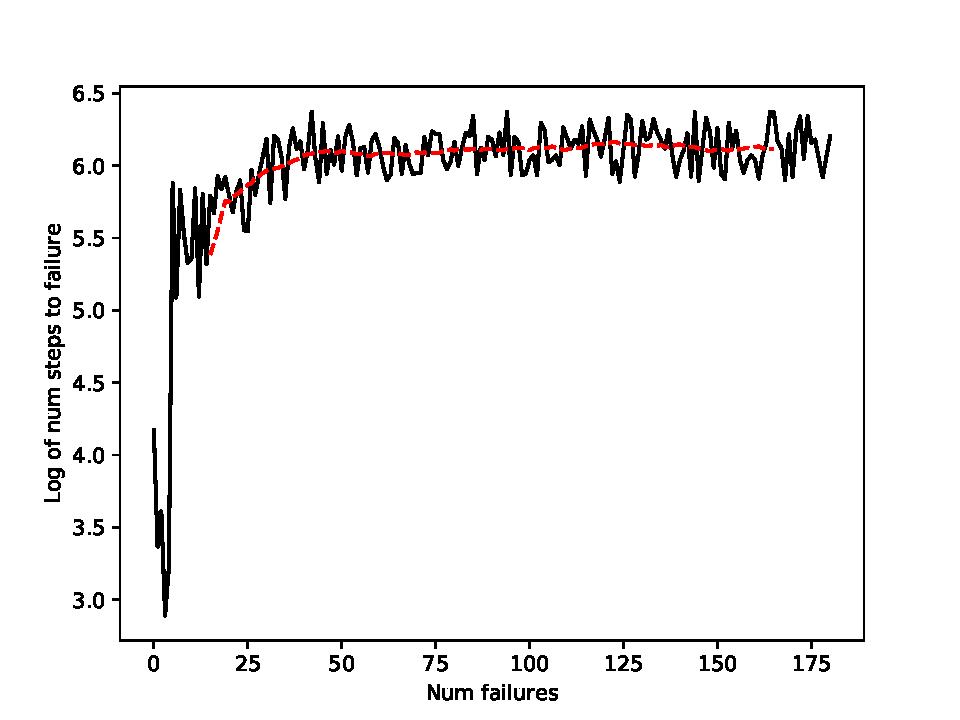
\includegraphics[width=\linewidth]{src/cartpole/control.pdf}
	\end{figure}
	
	\newpage
	\section{Problem 2: KL Divergence and Maximum Likelihood}
	\subsection{(a) Non-negativity}
	\begin{proof}
		Show:
		\begin{align}
			\forall P, Q, D_{KL}(P||Q) \geq 0
		\end{align}
		Let $P, Q$ characterize two arbitrary distributions over $\mc{X}$,
		\begin{align}
			D_{KL}(P||Q) &:= \sum_{x \in \mc{X}} P(x) \log \frac{P(x)}{Q(x)} \\
			&= \sum_{x \in \mc{X}} P(x) \left(-\log \frac{Q(x)}{P(x)} \right)\\
			&= \mathbb{E}_{x \sim P} \left [
			- \log \frac{Q(x)}{P(x)}
			\right ]
		\end{align}
		Since $-\log(\cdot)$ is a convex function, by Jensen's inequality
		\begin{align}
			\mathbb{E}_{x \sim P} \left [
			- \log \frac{Q(x)}{P(x)}
			\right ] &\geq -\log \left (
			\mathbb{E}_{x \sim P} \left [
			\frac{Q(x)}{P(x)}
			\right]
			\right ) \\
			&= - \log \left(
			\sum_{x \in \mc{X}}P(x) \frac{Q(x)}{P(x)}
			\right ) \\
			&= - \log \left(
			\sum_{x \in \mc{X}}Q(x)
			\right ) \\
			&= - \log(1) \because \tx{ $Q(\cdot)$ is a distribution} \\
			&= 0
		\end{align}
		Therefore,
		\begin{align}
			D_{KL}(P||Q) \geq 0
		\end{align}
		Show 
		\begin{align}
			D_{KL}(P||Q) = 0 \impliedby P = Q
		\end{align}
		Suppose $P(x) = Q(x)$ for every $x \in \mc{X}$,
		\begin{align}
			D_{KL}(P||Q) &= \sum_{x \in \mc{X}} P(x) \log(1) \\
			&= \sum_{x \in \mc{X}} P(x)\ 0 = 0
		\end{align}
		Show
		\begin{align}
			D_{KL}(P||Q) = 0 \implies P = Q
		\end{align}
		Note that the second part of Jensen's inequality suggested that the equality, $D_{KL}(P||Q) = 0$ implies $-\log \frac{Q(x)}{P(x)}$ is constant over $\mc{X}$. Also, since $-\log(\cdot)$ is in fact injective, so it must be the case that $\frac{Q(x)}{P(x)}$ is constant over $\mc{X}$. Therefore, $\mathbb{E}_{x \sim P} \left [\frac{Q(x)}{P(x)} \right] = \frac{P(c)}{Q(c)}$ for every $c \in \mc{X}$. Further, because $\mathbb{E}_{x \sim P} \left [\frac{Q(x)}{P(x)} \right] = \sum_{x \in \mc{X}} P(x) \frac{Q(x)}{P(x)} = \sum_{x \in \mc{X}} Q(x)$, which equals one because $Q$ is a probability distribution over $\mc{X}$. Therefore, for every $c \in \mc{X}$, $P(c) = Q(c)$. That's, $P = Q$.
		
	\end{proof}
	
	\newpage
	\subsection{(b) Chain rule for KL divergence}
	\begin{proof}
		\begin{align}
		&D_{KL}(P(X) || Q(X)) + D_{KL}(P(Y|X)||Q(Y|X))\\
		&= \sum_x P(x) \log \frac{P(x)}{Q(x)} + \sum_y P(y) \sum_x P(x|y) \log \frac{P(x|y)}{Q(x|y)} \\
		&= \sum_x \left (\sum_y P(x, y) \right) \log \frac{P(x)}{Q(x)} + \sum_y \sum_x P(y) P(x|y) \log \frac{P(x|y)}{Q(x|y)} \\
		&= \sum_{x, y} P(x, y) \log \frac{P(x)}{Q(x)} + \sum_{x, y} P(x, y) \log \frac{P(x|y)}{Q(x|y)} \\
		&= \sum_{x, y} P(x, y) \log \frac{P(x)}{Q(x)} + \log \frac{P(x|y)}{Q(x|y)} \\
		&= \sum_{x, y} P(x, y) \log \frac{P(x)P(x|y)}{Q(x)Q(x|y)}\\
		&= \sum_{x, y} P(x, y) \log \frac{P(x, y)}{Q(x, y)} \\
		&= D_{KL}(P(X,Y)||Q(X,Y))
		\end{align}
	\end{proof}
	
	\newpage
	\subsection{(c) KL and maximum likelihood}
	\begin{proof}
		Let $\mc{M}$ denote the support of $\hat{P}$ (indeed, $\mc{M}$ is the set of distinct elements in dataset $\{x\upi\}_{i=1}^n$), which is a subset of support of $P_\theta$.
		\begin{align}
			\argmin_\theta D_{KL}(\hat{P}||P_\theta) &= \argmin_\theta \sum_{x \in \mc{M}} \hat{P}(x) \log \frac{\hat{P}(x)}{P_\theta(x)} \\
			&= \argmin_\theta \underbrace{\sum_{x \in \mc{M}} \hat{P}(x) \log \hat{P}(x)}_{\perp \theta} - \sum_{x \in \mc{M}} \hat{P}(x) \log P_\theta(x) \\
			&= \argmin_\theta - \sum_{x \in \mc{M}} \hat{P}(x) \log P_\theta(x) \\
			&= \argmax_\theta  \sum_{x \in \mc{M}} \hat{P}(x) \log P_\theta(x) \\
			&= \argmax_\theta \sum_{x \in \mc{M}}\left( \frac{1}{n} \sum_{i=1}^n \id{x\upi = x} \right ) \log P_\theta(x) \\
			&= \argmax_\theta \frac{1}{n} \sum_{x \in \mc{M}}\left( \sum_{i=1}^n \id{x\upi = x} \right ) \log P_\theta(x) 
		\end{align}
		For each $x \in \mc{M}$, $\sum_{i=1}^n \id{x\upi = x}$ in fact counts the number of occurrences of $x$ in dataset $\{x\upi\}_{i=1}^n$. Therefore, the scope of summation above can be transformed from $\mc{M}$ to $\{x\upi\}_{i=1}^n$, by dropping the occurrence counting multiplier $\sum_{i=1}^n \id{x\upi = x}$.\footnote{This can be easily verified by writing out all terms in the summation.} Hence,
		\begin{align}
			\argmax_\theta \frac{1}{n} \sum_{x \in \mc{M}}\left( \sum_{i=1}^n \id{x\upi = x} \right ) \log P_\theta(x) &= \frac{1}{n} \sum_{i=1}^n \log P_\theta (x\upi)
		\end{align}
		Dropping the positive term $\frac{1}{n}$ does not affect the maximizer. Therefore,
		\begin{align}
			\argmin_\theta D_{KL}(\hat{P}||P_\theta) &= \argmax_\theta \sum_{i=1}^n \log P_\theta (x\upi)
		\end{align}
	\end{proof}
	
	\newpage
	\section{Problem 3: K-means for Compression}
	\subsection{(a) K-Means Compression Implementation}
	\begin{figure}[H]
		\centering
		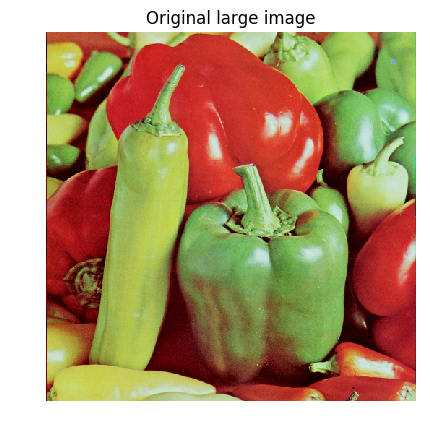
\includegraphics[width=\linewidth]{src/k_means/orig_large.png}
		\caption{Original Large}
	\end{figure}
	
	\begin{figure}[H]
		\centering
		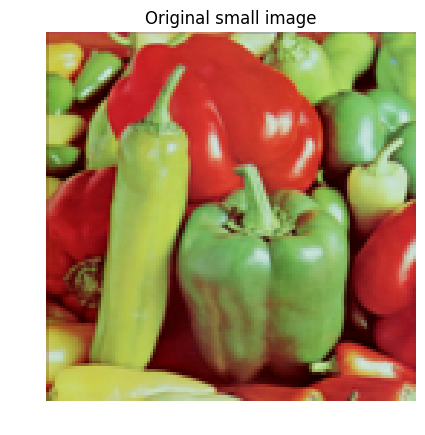
\includegraphics[width=\linewidth]{src/k_means/orig_small.png}
		\caption{Original Small}
	\end{figure}
	
	\begin{figure}[H]
		\centering
		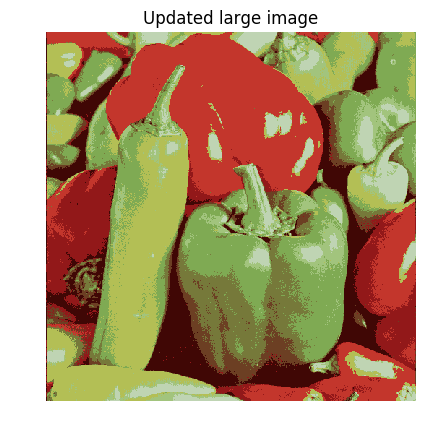
\includegraphics[width=\linewidth]{src/k_means/updated_large.png}
		\caption{Compressed Large}
	\end{figure}
	
	\newpage
	\subsection{(b) Compression Factor}
	\paragraph{Answer} In the original 8-bit 3-channel representation, each pixel requires $3 \times 8 = 24$ bits to be fully characterized. In the compressed representation, each pixel can be mapped to one of 16 clusters indexed by 0 to 15. To represent which cluster one particular pixel belongs to, one would need 4-bits (from 0000 to 1111). Therefore, images are compressed by factor of $\frac{24}{4} = 6$.
	
	\newpage
	\section{Problem 4: Semi-supervised EM}
	\subsection{(a) Convergence}
	\begin{proof}
		\begin{align}
			\ell_{\tx{semi-sup}}(\theta^{(t+1)}) &= \ell_{\tx{unsup}}(\theta^{(t+1)}) + \alpha \ell_{\tx{sup}}(\theta^{(t+1)}) \\
			&= \sum_{i=1}^n \log \left(
			\sum_{z\upi} Q^{(t)}_i \frac{p(x\upi, z\upi; \theta^{(t+1)})}{Q^{(t)}_i}
			\right) + \alpha \ell_{\tx{sup}}(\theta^{(t+1)}) \\
			&= \sum_{i=1}^n \log \mathbb{E}_{z\upi \sim Q^{(t)}_i} \left[\frac{p(x\upi, z\upi; \theta^{(t+1)})}{Q^{(t)}_i}\right] + \alpha \ell_{\tx{sup}}(\theta^{(t+1)}) \\
			&\geq \sum_{i=1}^n \mathbb{E}_{z\upi \sim Q^{(t)}_i} \left[\log \frac{p(x\upi, z\upi; \theta^{(t+1)})}{Q^{(t)}_i}\right] + \alpha \ell_{\tx{sup}}(\theta^{(t+1)}) \because \tx{Jensen's Inequality} \\
			&= \sum_{i=1}^n \sum_{z\upi} Q^{(t)}_i \log \left( \frac{p(x\upi, z\upi; \theta^{(t+1)})}{Q^{(t)}_i}\right ) + \alpha \ell_{\tx{sup}}(\theta^{(t+1)}) \\
			&\geq \sum_{i=1}^n \sum_{z\upi} Q^{(t)}_i \log \left( \frac{p(x\upi, z\upi; \theta^{(t)})}{Q^{(t)}_i}\right ) + \alpha \ell_{\tx{sup}}(\theta^{(t)}) \because \tx{M-step is maximizing w.r.t. $\theta$} \\
			&= \sum_{i=1}^n \log \left( \sum_{z\upi} Q^{(t)}_i \frac{p(x\upi, z\upi; \theta^{(t)})}{Q^{(t)}_i}\right ) + \alpha \ell_{\tx{sup}}(\theta^{(t)}) \\
			&= \ell_{\tx{semi-sup}}(\theta^{(t)})
		\end{align}
		The last two steps were derive from the fact that $Q(\cdot)$ was specifically chosen in the E-step so that $\ell_{\tx{semi-sup}}(\theta^{(t)})$ was equal to it's ELBO.
	\end{proof}
	
	\newpage
	\subsection{(b) Semi-supervised E-step}
	\paragraph{Answer} $z\upi$ for all unlabelled examples should be estimated. Specifically, posterior $p(z\upi | x\upi; \mu, \Sigma, \phi)$ for all $i \in \{1,\cdots,n\}$ are estimated. Define $w\upi_j = p(z\upi = j | x\upi; \mu, \Sigma, \phi)$.
	\begin{proof}
		\begin{align}
		w\upi_j &:= p(z\upi = j| x\upi; \mu, \Sigma, \phi) \\
		&= \frac{p(x\upi|z\upi = j; \mu, \Sigma, \phi) p(z\upi = j; \mu, \Sigma, \phi)}{p(x\upi; \mu, \Sigma, \phi)} \\
		&= \frac{p(x\upi|z\upi = j; \mu, \Sigma, \phi) p(z\upi = j; \mu, \Sigma, \phi)}{\sum_{\ell=1}^k \left \{p(x\upi|z\upi = \ell; \mu, \Sigma, \phi) p(z\upi = \ell; \mu, \Sigma, \phi) \right\}} \\
		&= \frac{
		 \frac{1}{(2\pi)^{d/2} |\Sigma_j|^{1/2}} \exp \left[
		 	- \frac{1}{2} (x\upi - \mu_j)^T \Sigma_j^{-1} (x\upi - \mu_j) \right] \phi_j
		}{
		 \sum_{\ell=1}^k \left\{
		 	\frac{1}{(2\pi)^{d/2} |\Sigma_\ell|^{1/2}} \exp \left[
		 	- \frac{1}{2} (x\upi - \mu_\ell)^T \Sigma_\ell^{-1} (x\upi - \mu_\ell)\right] \phi_\ell
		 \right\}
		}
		\end{align}
	\end{proof}
	
	\newpage
	\subsection{(c) Semi-supervised M-step}
	\subsubsection{Choosing $\mu_\ell^{(t+1)}$}
	\paragraph{Answer} Let $\Theta := \{\mu_\ell, \Sigma_\ell, \phi_\ell\}_{\ell=1}^k$. The first order condition is for optimal $\mu_\ell$ is:
	\begin{proof}
		\begin{align}
			\nabla{\mu_\ell}\ \ell_{\tx{semi-sup}}(\Theta) &= \nabla{\mu_\ell}\ \sum_{i=1}^n \sum_{j=1}^k w\upi_j \log \left( \frac{p(x\upi, z\upi; \Theta)}{w\upi_j} \right) + \alpha \sum_{i=1}^{\tilde{n}} \log \left(p(\tilde{x}\upi, \tilde{z}\upi; \Theta)
			\right) \\
			&= \nabla_{\mu_\ell}\ \sum_{i=1}^n w\upi_\ell \log \left( \frac{p(x\upi, z\upi; \Theta)}{w\upi_\ell} \right) + \alpha \sum_{i=1}^{\tilde{n}} \id{\tilde{z}\upi = \ell} \log \left(p(\tilde{x}\upi, \tilde{z}\upi; \Theta) \right) \\
			&= \nabla_{\mu_\ell}\ \sum_{i=1}^n w\upi_\ell \log \left(p(x\upi, z\upi; \Theta) \right) + \alpha \sum_{i=1}^{\tilde{n}} \id{\tilde{z}\upi = \ell} \log \left(p(\tilde{x}\upi, \tilde{z}\upi; \Theta) \right) \\
			&= \nabla_{\mu_\ell}\ \sum_{i=1}^n w\upi_\ell \log \left(p(x\upi | z\upi; \Theta) p(z\upi; \Theta) \right) + \alpha \sum_{i=1}^{\tilde{n}} \id{\tilde{z}\upi = \ell} \log \left(p(\tilde{x}\upi | \tilde{z}\upi; \Theta) p(\tilde{z}\upi; \Theta) \right) \\
			&= \nabla_{\mu_\ell}\ \sum_{i=1}^n w\upi_\ell \left \{
			\log \left(
			p(x\upi|z\upi; \Theta)
			\right )
			\right\} + \alpha \sum_{i=1}^{\tilde{n}} \id{\tilde{z}\upi = \ell} \log \left(p(\tilde{x}\upi | \tilde{z}\upi; \Theta) \right) \\
			&= \nabla_{\mu_\ell}\ \sum_{i=1}^n w\upi_\ell \left \{- \frac{1}{2} (x\upi - \mu_\ell)^T \Sigma^{-1}_\ell (x\upi - \mu_\ell) \right \} \\
			&+ \alpha \sum_{i=1}^{\tilde{n}} \id{\tilde{z}\upi = \ell} \left \{
			-\frac{1}{2} (\tilde{x}\upi - \mu_\ell)^T \Sigma^{-1}_\ell (\tilde{x}\upi - \mu_\ell)
			\right \} \\
			&= \sum_{i=1}^n w\upi_\ell \left \{
			x^{(i)T} \Sigma^{-1}_\ell - \mu_\ell^T \Sigma^{-1}_\ell
			\right\} + \alpha \sum_{i=1}^{\tilde{n}} \id{\tilde{z}\upi = \ell} \left \{
			\tilde{x}^{(i)T} \Sigma^{-1}_\ell - \mu_\ell^T \Sigma^{-1}_\ell
			\right\} \\
			&= 0
		\end{align}
		By right multiplying $\Sigma_\ell^{-1}$,
		\begin{align}
			\sum_{i=1}^n w\upi_\ell \left \{
			x\upi - \mu_\ell
			\right\} + \alpha \sum_{i=1}^{\tilde{n}} \id{\tilde{z}\upi = \ell} \left \{
			\tilde{x}\upi - \mu_\ell
			\right\} &= 0 \\
			\implies \mu_\ell = \frac{\sum_{i=1}^n w_\ell\upi x\upi + \alpha \sum_{i=1}^{\tilde{n}} \id{\tilde{z}\upi = \ell} \tilde{x}\upi}{\sum_{i=1}^n w_\ell\upi + \alpha \sum_{i=1}^{\tilde{n}} \id{\tilde{z}\upi = \ell}}
		\end{align}
	\end{proof}
	\subsubsection{Choosing $\Sigma_\ell$}
	\begin{proof}
		Let $S_\ell := \Sigma_\ell^{-1}$. From lecture we know that the first order condition of optimizing $\Sigma_\ell$ is the same as finding the first order condition for $S_\ell$.
		\begin{align}
			\nabla_{S_\ell}\ \ell_{\tx{semi-sup}}(\Theta) &= \nabla_{S_\ell}\ \sum_{i=1}^n \sum_{j=1}^k w\upi_j \log \left( \frac{p(x\upi, z\upi; \Theta)}{w\upi_j} \right) + \alpha \sum_{i=1}^{\tilde{n}} \log \left(p(\tilde{x}\upi, \tilde{z}\upi; \Theta)
			\right) \\
			&= \nabla_{S_\ell}\ \sum_{i=1}^n w\upi_\ell \log \left( \frac{p(x\upi, z\upi; \Theta)}{w\upi_\ell} \right) + \alpha \sum_{i=1}^{\tilde{n}} \id{\tilde{z}\upi = \ell} \log \left(p(\tilde{x}\upi, \tilde{z}\upi; \Theta) \right) \\
			&= \nabla_{S_\ell} \sum_{i=1}^n w_\ell\upi \left(
			\log(|\Sigma_\ell|^{-1}) - \frac{1}{2} (x\upi - \mu_\ell)^T S_\ell (x\upi - \mu_\ell) \right) \\
			&+ \alpha \sum_{i=1}^{\tilde{n}} \id{\tilde{z}\upi = \ell} \left (
				\log(|\Sigma_\ell|^{-1}) - \frac{1}{2} (\tilde{x}\upi - \mu_\ell)^T S_\ell (\tilde{x}\upi - \mu_\ell)
			\right) \\
			&= \nabla_{S_\ell} \sum_{i=1}^n w_\ell\upi \left(
			\log(|S_\ell|) - \frac{1}{2} (x\upi - \mu_\ell)^T S_\ell (x\upi - \mu_\ell) \right) \\
			&+ \alpha \sum_{i=1}^{\tilde{n}} \id{\tilde{z}\upi = \ell} \left (
				\log(|S_\ell|) - \frac{1}{2} (\tilde{x}\upi - \mu_\ell)^T S_\ell (\tilde{x}\upi - \mu_\ell)
			\right) \\
			&= \sum_{i=1}^n w_\ell\upi S_\ell^{-T} - w_\ell\upi (x\upi - \mu_\ell) (x\upi - \mu_\ell)^T + \alpha \sum_{i=1}^{\tilde{n}} \id{\tilde{z}\upi = \ell} \left(
			S_\ell^{-T} - (\tilde{x}\upi - u_\ell) (\tilde{x}\upi - u_\ell)^T
			\right) \\
			&= 0
		\end{align}
		Since $\Sigma_\ell$ is symmetric, so $S^{-T}_\ell = \Sigma_\ell$. Above first order condition implies
		\begin{align}
			\Sigma_\ell \left (\sum_{i=1}^n w_\ell\upi + \alpha \sum_{i=1}^{\tilde{n}} \id{\tilde{z}\upi = \ell} \right) = \sum_{i=1}^n w_\ell\upi (x\upi - \mu_\ell) (x\upi - \mu_\ell)^T + \alpha \sum_{i=1}^{\tilde{n}} \id{\tilde{z}\upi = \ell} (\tilde{x}\upi - u_\ell) (\tilde{x}\upi - u_\ell)^T \\
			\implies \Sigma_\ell = \frac{\sum_{i=1}^n w_\ell\upi (x\upi - \mu_\ell) (x\upi - \mu_\ell)^T + \alpha \sum_{i=1}^{\tilde{n}} \id{\tilde{z}\upi = \ell} (\tilde{x}\upi - u_\ell) (\tilde{x}\upi - u_\ell)^T}{\sum_{i=1}^n w_\ell\upi + \alpha \sum_{i=1}^{\tilde{n}} \id{\tilde{z}\upi = \ell}}
		\end{align}
	\end{proof}
	\subsubsection{Choosing $\phi_\ell$}
	\begin{proof}
		\begin{align}
		\nabla_{\phi_\ell} \ell_{\tx{semi-sup}}(\Theta) &= \nabla_{\phi_\ell} \sum_{i=1}^n \sum_{\ell=1}^k w_\ell\upi \log \left(
		\frac{p(x\upi|z\upi=\ell; \Theta)p(z\upi=\ell; \Theta)}{p(x\upi|z\upi=\ell; \Theta)}
		\right)
		+ \alpha \sum_{i=1}^{\tilde{n}} \log \left(p(\tilde{x}\upi| \tilde{z}\upi; \Theta) p(\tilde{z}; \Theta) \right) \\
		&= \nabla_{\phi_\ell} \sum_{i=1}^n \sum_{\ell=1}^k w_\ell\upi \log \left( p(z\upi = \ell; \Theta) \right)
		+ \alpha \sum_{i=1}^{\tilde{n}} \id{\tilde{z}\upi = \ell}\log (\phi_\ell) \\
		&= \nabla_{\phi_\ell} \sum_{i=1}^n \sum_{\ell=1}^k w_\ell\upi \log (\phi_\ell)
		+ \alpha \sum_{i=1}^{\tilde{n}} \id{\tilde{z}\upi = \ell}\log (\phi_\ell) \\
		&= \nabla_{\phi_\ell} \sum_{i=1}^n w_\ell\upi \log (\phi_\ell)
		+ \alpha \sum_{i=1}^{\tilde{n}} \id{\tilde{z}\upi = \ell}\log (\phi_\ell)
		\end{align}
		Using the constraint that $\sum_{\ell=1}^k \phi_\ell = 1$, the Lagrangian can be constructed as
		\begin{align}
			\mc{L}(\cdot) &= \ell_{\tx{semi-sup}}(\phi, \cdot) + \lambda \left(1 - \sum_{\ell=1}^k \phi_\ell \right)
		\end{align}
		Solving the stationary point for $\mc{L}(\cdot)$ gives
		\begin{align}
			\pd{\mc{L}(\phi_\ell, \cdot)}{\phi_\ell} &= \nabla_{\phi_\ell} \ell_{\tx{semi-sup}} - \lambda \\
			&= \frac{1}{\phi_\ell} \left (
			\sum_{i=1}^n w_\ell\upi + \alpha \sum_{i=1}^{\tilde{n}}
			\id{\tilde{z}\upi = \ell} \right) - \lambda = 0\\
			& \implies \frac{1}{\lambda} \left (
			\sum_{i=1}^n w_\ell\upi + \alpha \sum_{i=1}^{\tilde{n}}
			\id{\tilde{z}\upi = \ell} \right) = \phi_\ell
		\end{align}
		Then, $\sum_{\ell=1}^k \phi_\ell = 1$ implies
		\begin{align}
			\sum_{\ell=1}^k \frac{1}{\lambda} \left (
			\sum_{i=1}^n w_\ell\upi + \alpha \sum_{i=1}^{\tilde{n}}
			\id{\tilde{z}\upi = \ell} \right) &= 1 \\
			\implies \sum_{\ell=1}^k \left (
			\sum_{i=1}^n w_\ell\upi + \alpha \sum_{i=1}^{\tilde{n}}
			\id{\tilde{z}\upi = \ell} \right) &= \lambda
		\end{align}
		Therefore, 
		\begin{align}
			\phi_\ell &= \frac{
			\sum_{i=1}^n w_\ell\upi + \alpha \sum_{i=1}^{\tilde{n}}
			\id{\tilde{z}\upi = \ell}
			}{
			\sum_{j=1}^k \left (
			\sum_{i=1}^n w_j\upi + \alpha \sum_{i=1}^{\tilde{n}}
			\id{\tilde{z}\upi = j} \right)
			} \\
			&= \frac{
			\sum_{i=1}^n w_\ell\upi + \alpha \sum_{i=1}^{\tilde{n}}
			\id{\tilde{z}\upi = \ell}
			}{
			\sum_{j=1}^k \sum_{i=1}^n w\upi_j
			+ \alpha \sum_{j=1}^k \sum_{i=1}^{\tilde{n}} \id{\tilde{z}\upi = j}
			} \\
			&= \frac{
			\sum_{i=1}^n w_\ell\upi + \alpha \sum_{i=1}^{\tilde{n}}
			\id{\tilde{z}\upi = \ell}
			}{
			\sum_{i=1}^n \sum_{j=1}^k w\upi_j
			+ \alpha \sum_{i=1}^{\tilde{n}} \sum_{j=1}^k \id{\tilde{z}\upi = j}
			} \\
			&= \frac{
			\sum_{i=1}^n w_\ell\upi + \alpha \sum_{i=1}^{\tilde{n}}
			\id{\tilde{z}\upi = \ell}
			}{
			n + \alpha \tilde{n}
			}
		\end{align}
	\end{proof}
	
	\newpage
	\subsection{(d) Classical (Unsupervised) EM Implememtation}
	\begin{figure}[H]
		\centering
		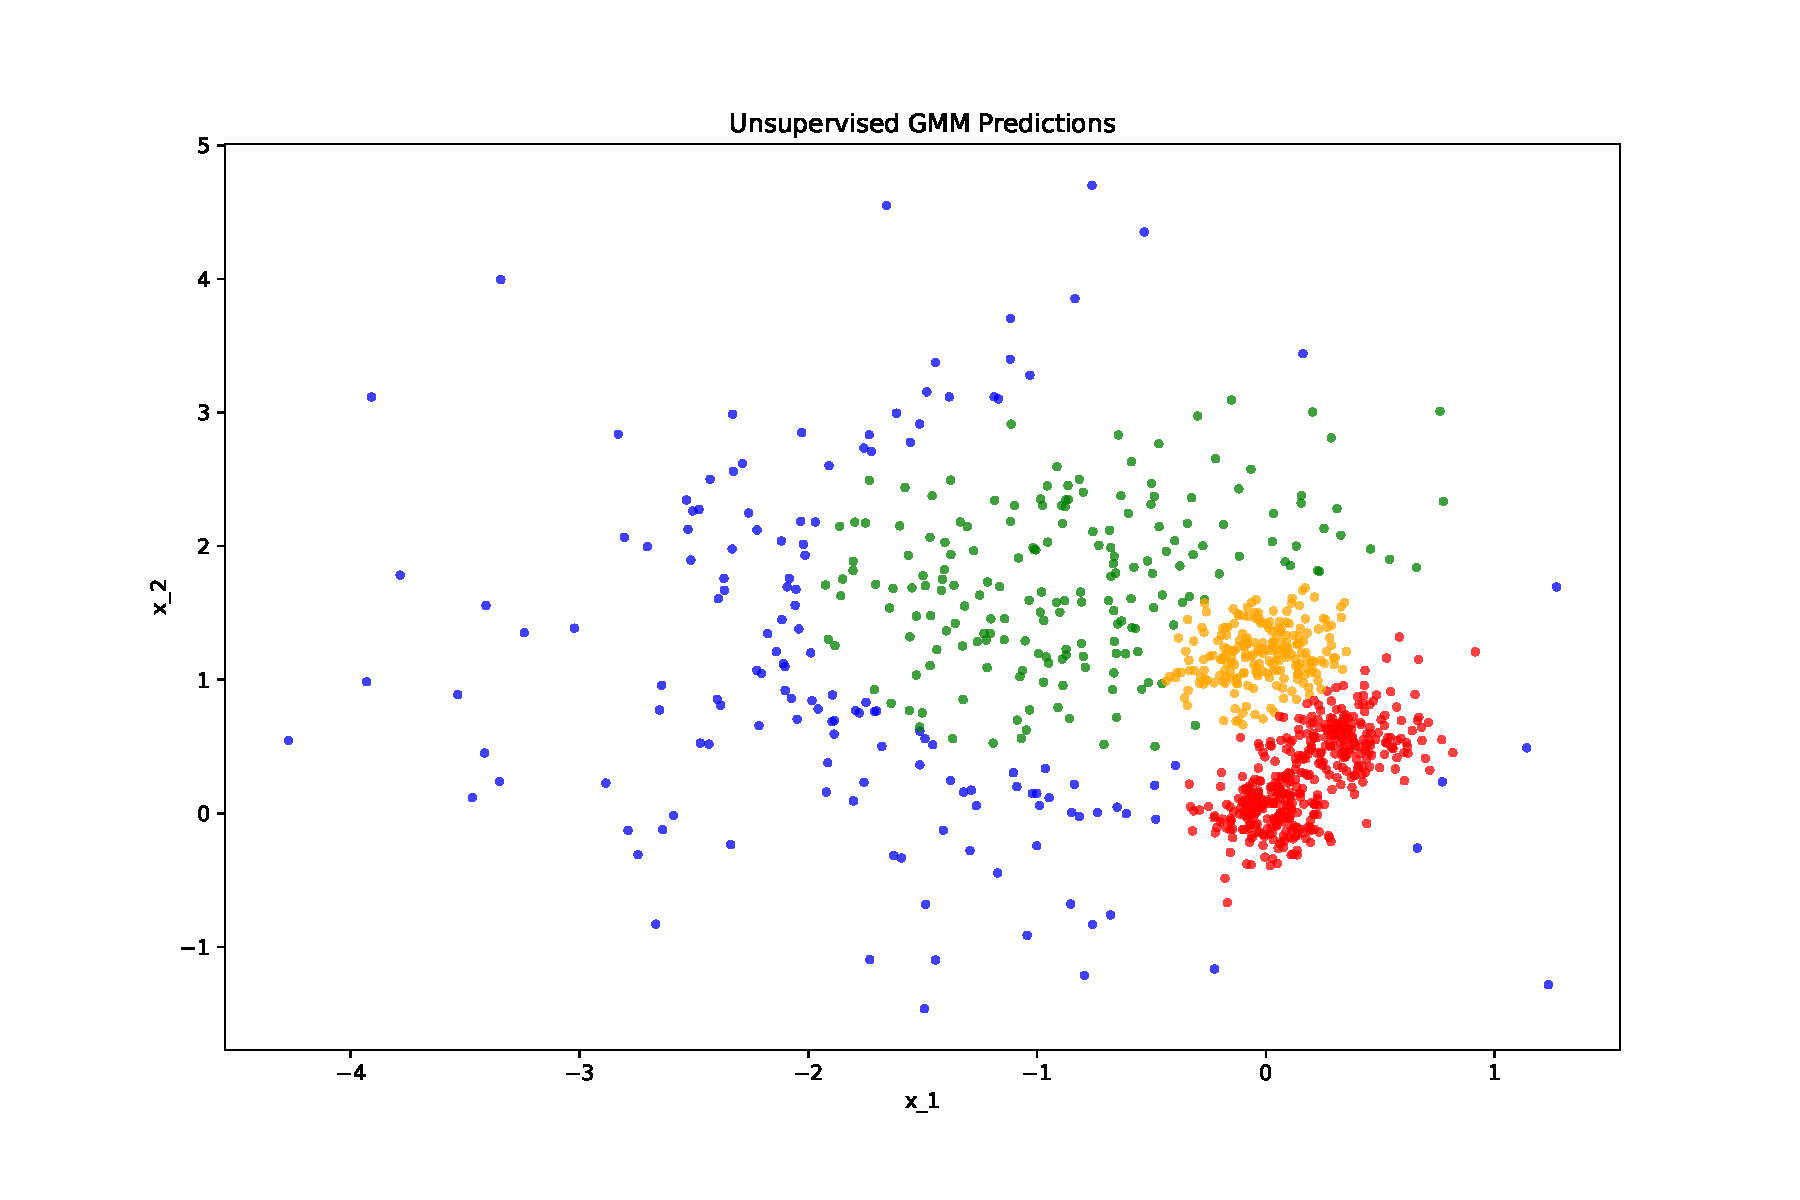
\includegraphics[width=\linewidth]{src/semi_supervised_em/pred_0.pdf}
	\end{figure}
	\begin{figure}[H]
		\centering
		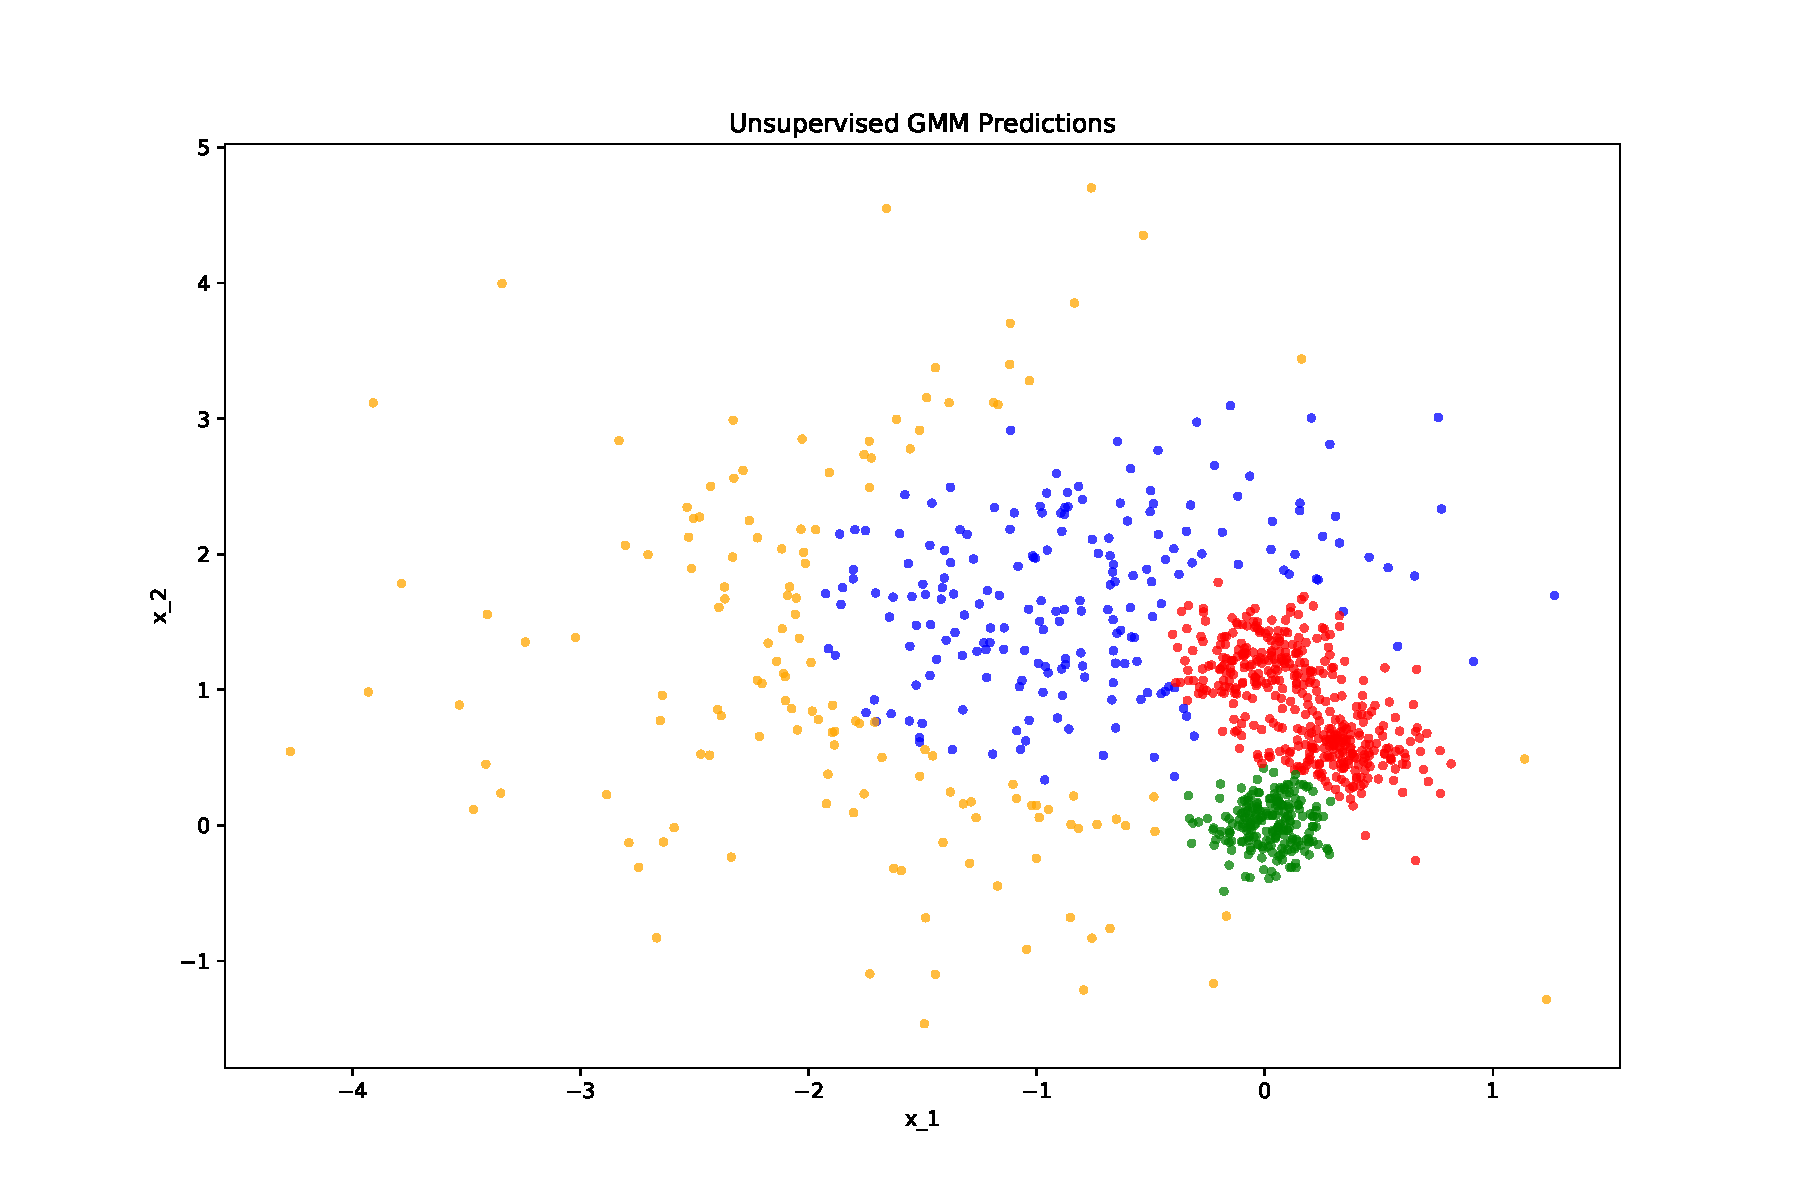
\includegraphics[width=\linewidth]{src/semi_supervised_em/pred_1.pdf}
	\end{figure}
	
	\begin{figure}[H]
		\centering
		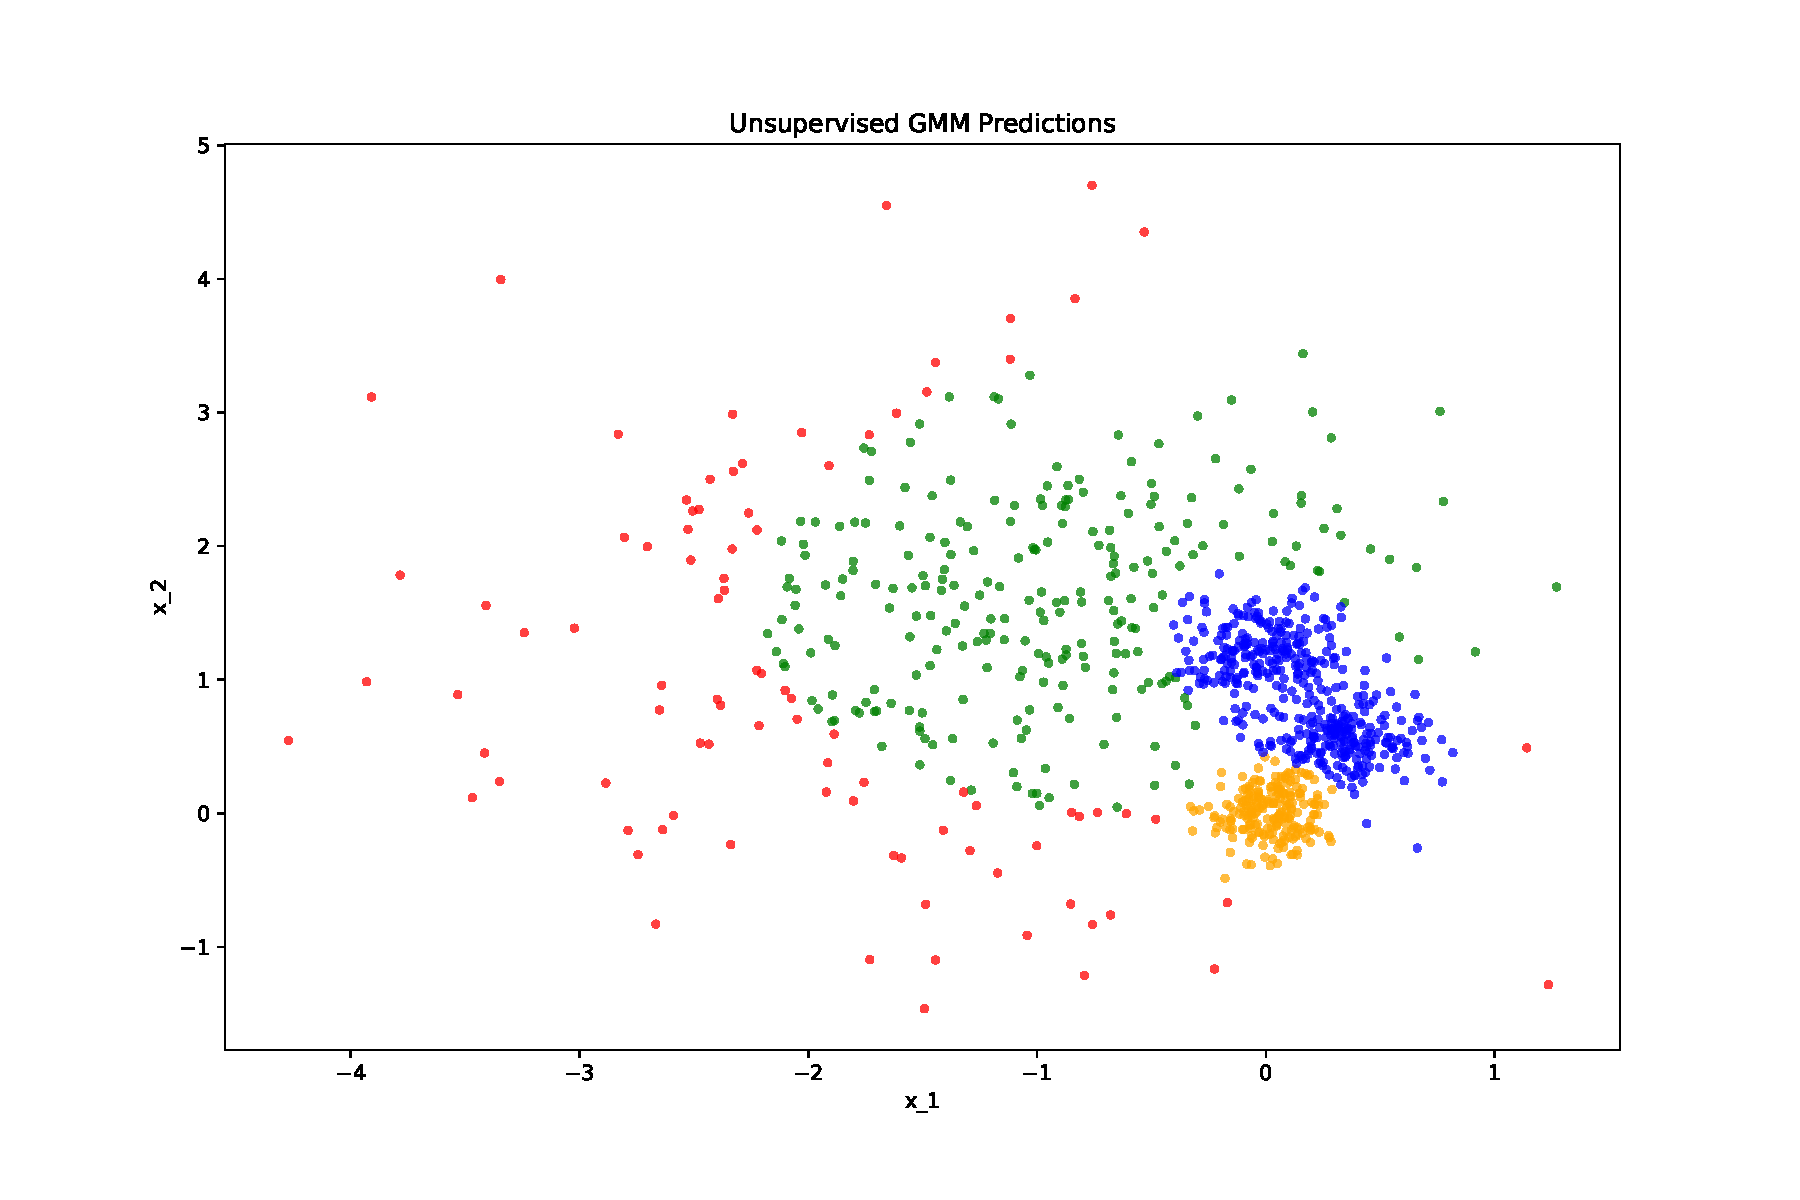
\includegraphics[width=\linewidth]{src/semi_supervised_em/pred_2.pdf}
	\end{figure}
	
	\newpage
	\subsection{(e) Semi-supervised EM Implementation}
	\begin{figure}[H]
		\centering
		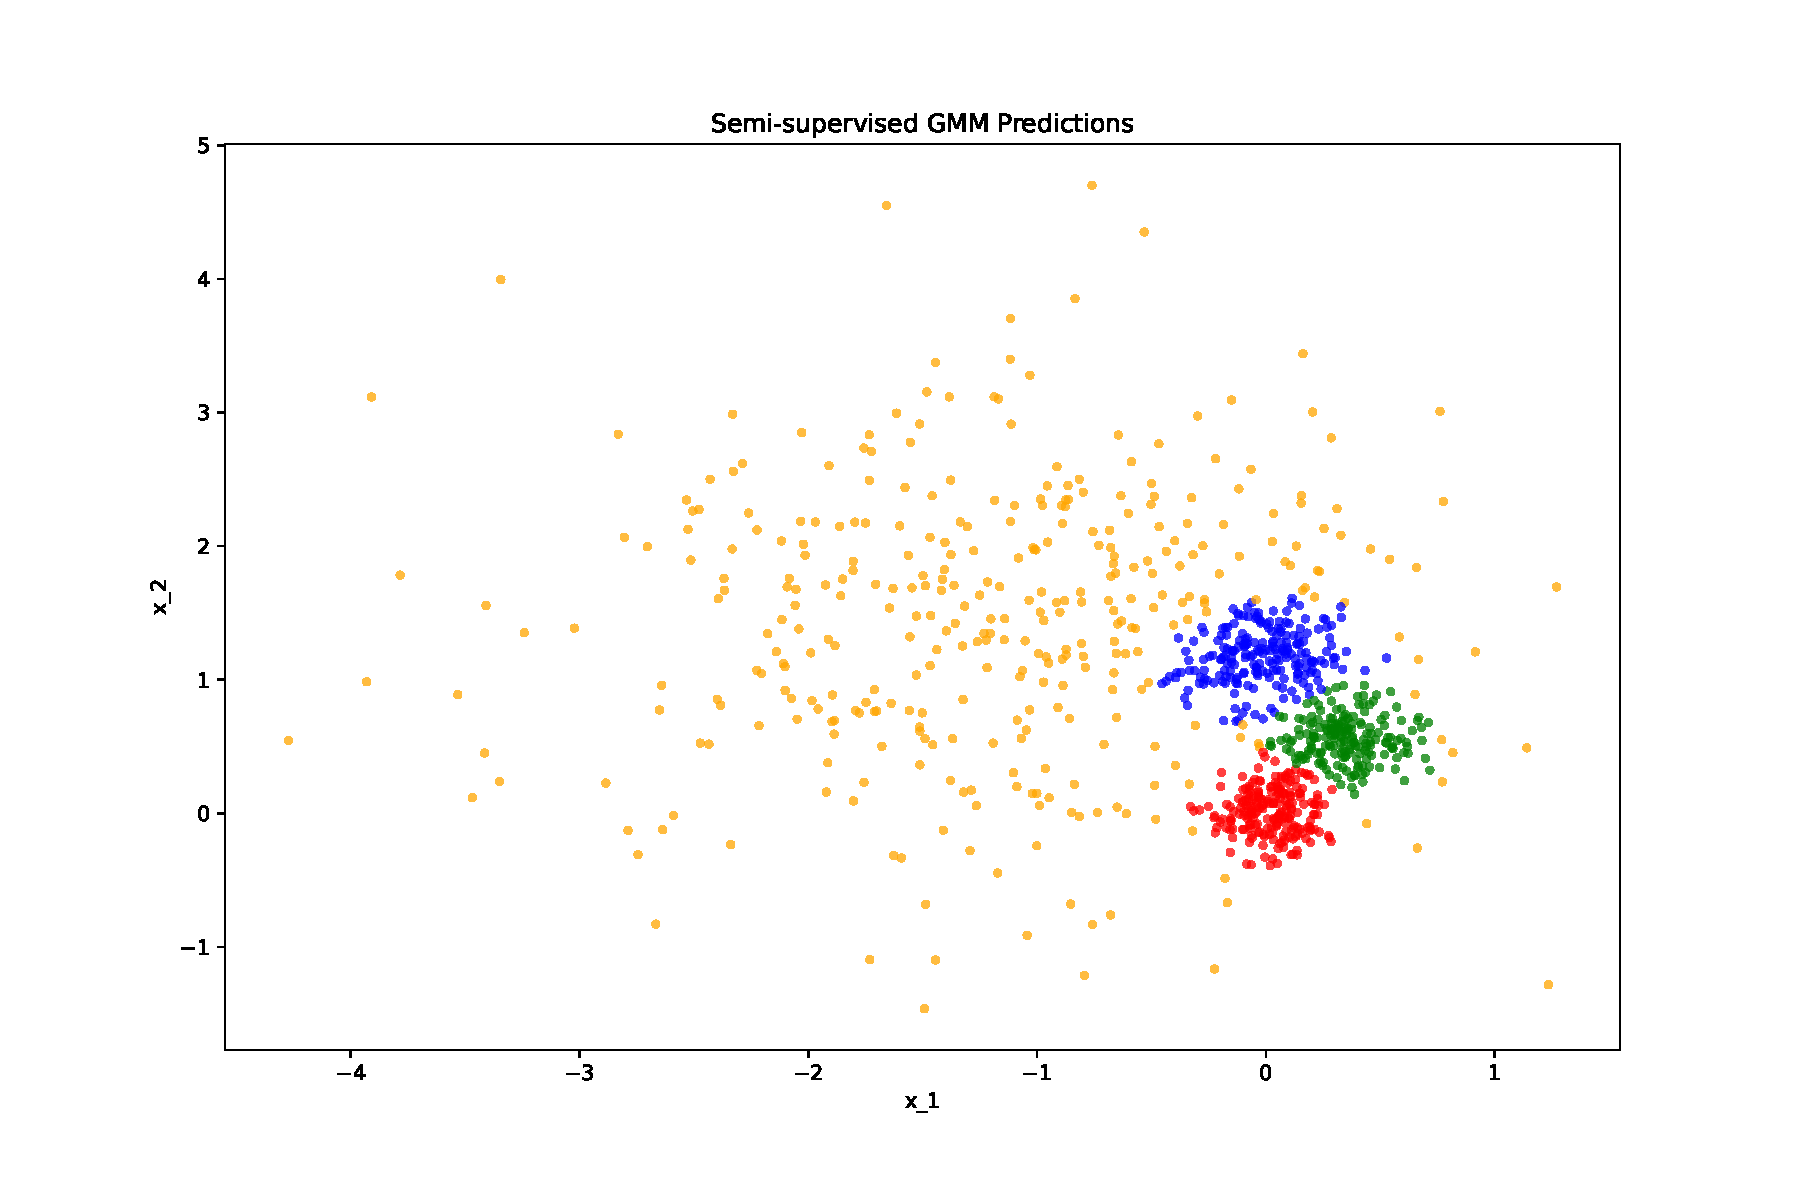
\includegraphics[width=\linewidth]{src/semi_supervised_em/pred_ss_0.pdf}
	\end{figure}
	\begin{figure}[H]
		\centering
		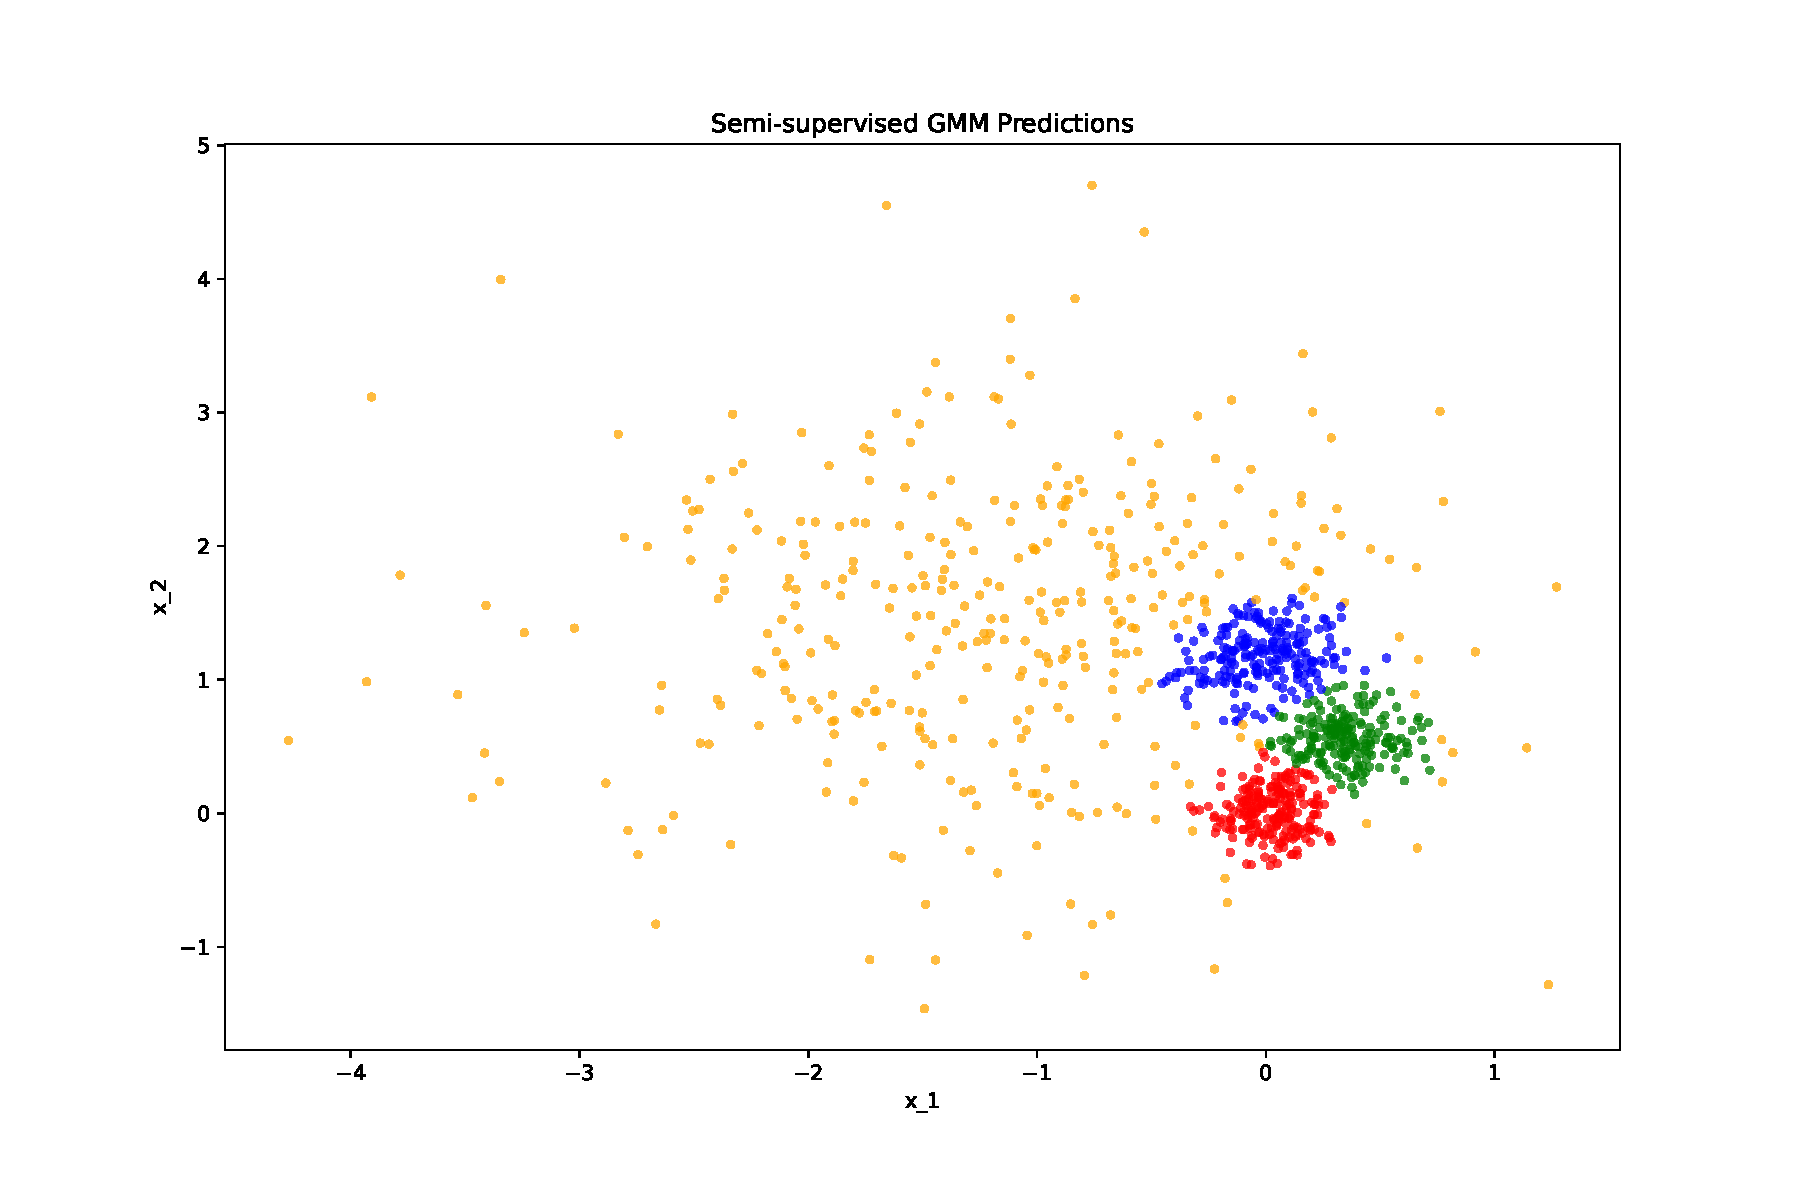
\includegraphics[width=\linewidth]{src/semi_supervised_em/pred_ss_1.pdf}
	\end{figure}
	\begin{figure}[H]
		\centering
		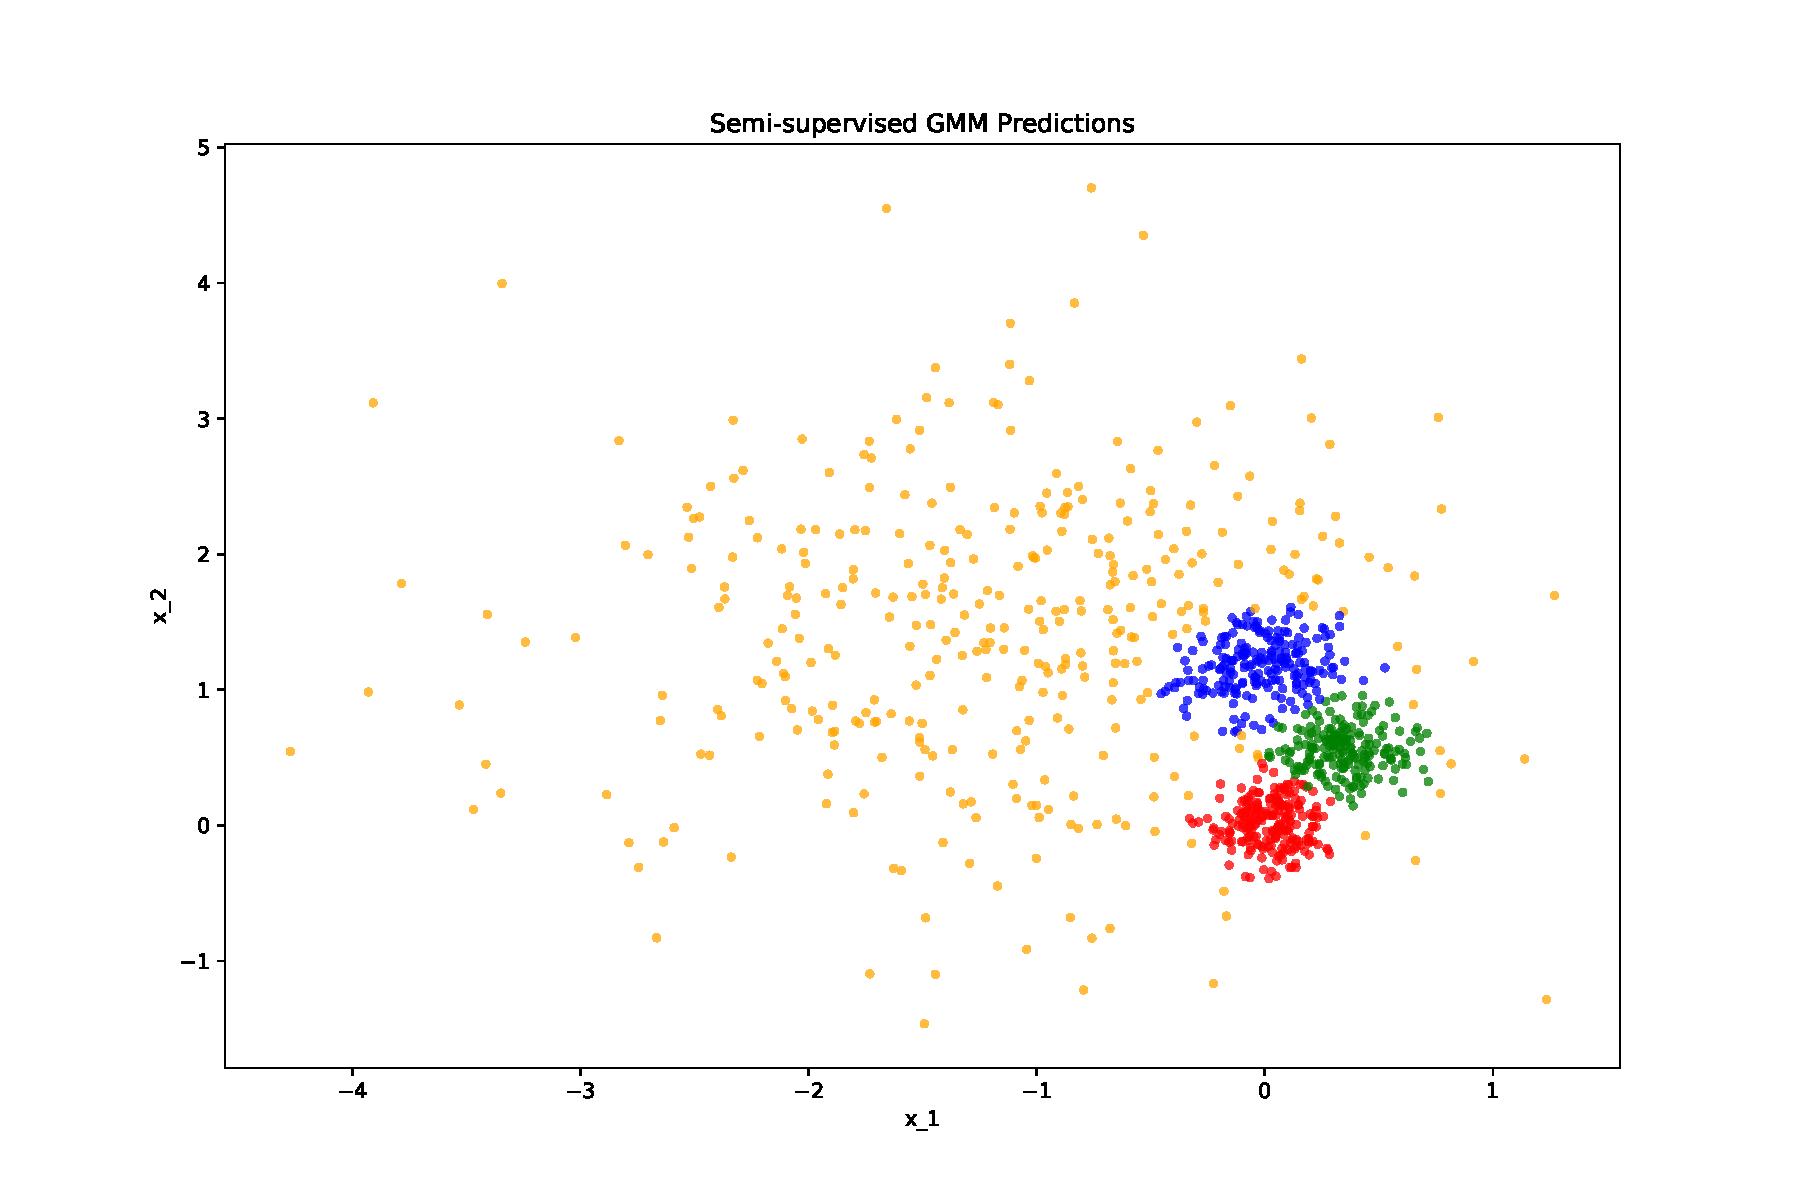
\includegraphics[width=\linewidth]{src/semi_supervised_em/pred_ss_2.pdf}
	\end{figure}
	
	\newpage
	\subsection{(f) Comparison}
	\paragraph{Answer}
	\begin{enumerate}
		\item The unsupervised GMM took more iterations (more than 100 iterations on average) to converge than the semi-supervised GMM took (around 25 iterations on average).
		\item Semi-supervised GMM was more stable than the unsupervised version, clusters were almost exactly (by looking at the clustering result, there were still couple of points changed) in all three experiments conducted. However, the clustering result for unsupervised GMM varied among three experiments.
		\item Given that the dataset was sampled from a mixture of three low-variance Gaussian distributions with one additional large variance Gaussian, the semi-supervised GMM successfully separated the the entire dataset into three low-variance groups and a fourth high-variance group. However, the unsupervised GMM clustered the dataset into two low-variance and two high-variance groups instead. Overall, the semi-supervised GMM provided higher quality results.
	\end{enumerate}
	
	\newpage
	\section{PCA}
	\begin{proof}
		Note that given a subspace $\mc{V} = \{\alpha u: \alpha \in \R\} \subset \R^d$ characterized by some unit vector $u$. Let $x \in \R^d$, $f_u(x)$ is defined to be the a vector in $\mc{V}$ closest to $x$. Indeed, $f_u(x)$ would be exactly the \emph{projection} of $x$ on $u$, which is given by
		\begin{align}
			f_u(x) = \frac{\inner{x}{u}}{\norm{u}^2_2} u = \inner{x}{u}u
		\end{align}
		because $u$ is a unit vector. Therefore,
		\begin{align}
			\argmin_{u: \norm{u}^2_2=1} \sum_{i=1}^n \norm{x\upi - f_u(x\upi)}^2_2 &= \argmin_{u: \norm{u}=1} \sum_{i=1}^n \norm{x\upi - \inner{x\upi}{u}u}^2_2 \\
			&= \argmin_{u: \norm{u}^2_2=1} \sum_{i=1}^n \left \langle
			x\upi - \inner{x\upi}{u}u,
			x\upi - \inner{x\upi}{u}u
			\right \rangle \\
			&= \argmin_{u: \norm{u}^2_2=1} \sum_{i=1}^n \left \langle x\upi, x\upi - \inner{x\upi}{u}u \right \rangle 
			- \left \langle \inner{x\upi}{u}u,
			x\upi - \inner{x\upi}{u}u \right \rangle \\
			&= \argmin_{u: \norm{u}^2_2=1} \sum_{i=1}^n \inner{x\upi}{x\upi}
			- 2 \left \langle
			x\upi, \inner{x\upi}{u}u
			\right \rangle
			+ \left \langle
			\inner{x\upi}{u}u,
			\inner{x\upi}{u}u
			\right \rangle \\
			&= \argmin_{u: \norm{u}^2_2=1} \sum_{i=1}^n \underbrace{\norm{x\upi}^2_2}_{\perp u}
			- 2 \inner{x\upi}{u} \inner{x\upi}{u}
			+ \inner{x\upi}{u}^2 \norm{u}^2_2 \\
			&= \argmin_{u: \norm{u}^2_2=1} \sum_{i=1}^n - 2  \inner{x\upi}{u}^2 +  \inner{x\upi}{u}^2 \\
			&= \argmax_{u: \norm{u}^2_2=1} \sum_{i=1}^n \inner{x\upi}{u}^2 \\
			&= \argmax_{u: \norm{u}^2_2=1} \sum_{i=1}^n u^T x\upi x^{(i)T} u \\
			&= \argmax_{u: \norm{u}^2_2=1} u^T \left(\sum_{i=1}^n x\upi x^{(i)T}\right) u \\
			&= \argmax_{u: \norm{u}^2_2=1} u^T \left(\frac{1}{n}\sum_{i=1}^n x\upi x^{(i)T}\right) u
		\end{align}
		where the last maximization is exactly the same as the maximization for choosing principal component on page 5 of the lecture notes for PCA.
	\end{proof}
	\newpage
	\section{Problem 6: Independent Components Analysis}
	\subsection{(a) Gaussian source}
	\begin{proof}
		Let $\phi(z)$ denote the PDF for $\mc{N}(0, 1)$.
		\begin{align}
			\nabla_W \ell(W) &= \nabla_W \sum_{i=1}^n \left(
			\log |W| + \sum_{j=1}^d \log \phi(w_j^T x\upi)
			\right) \\
			&= \sum_{i=1}^n \left(
			W^{-T} + \nabla_W \sum_{j=1}^d \log \phi (w_j^T x\upi)
			\right) \\
			&= \sum_{i=1}^n \left(
			W^{-T} + \nabla_W \sum_{j=1}^d \left (
			- \frac{1}{2} (w_j^T x\upi)^2
			\right)
			\right)
		\end{align}
		where the last step was derived by explicitly expanding $\phi(z)$ and dropping terms independent from $W$. Note that, for each $w_j$,
		\begin{align}
			\nabla_{w_j} \sum_{i=1}^n \sum_{j=1}^d \left (
			- \frac{1}{2} (w_j^T x\upi)^2 \right) &= - (w_j^T x\upi) x^{(i)T}
		\end{align}
		Gather results,
		\begin{align}
			\nabla_W \ell(W) &= n W^{-T} - \underbrace{\sum_{i=1}^n
			\begin{pmatrix}
				(w_1^T x\upi) x^{(i)T} \\
				(w_2^T x\upi) x^{(i)T} \\
				\vdots \\
				(w_j^T x\upi) x^{(i)T}
			\end{pmatrix}}_{:= \Omega \in \R^{d \times d}}
		\end{align}
		Claim: $\Omega = W X^T X$. This can be easily verified by considering the $(a, b)$ component of $\Omega$. $\Omega_{a, b} = \sum_{i=1}^n (w_a^T x\upi) x\upi_b = \sum_{i=1}^n \sum_{j=1}^d W_{a, j} x\upi_j x\upi_b$, which is exactly the same as  the $(a, b)$ component of $WX^TX$. Setting the gradient equal zero for the first order condition:
		\begin{align}
			\nabla_W \ell(W) = n W^{-T} - W X^T X =0 \\
			\implies W^T W = n \left(X^T X \right)^{-1}
		\end{align}
		Let $P \in \R^{d\times d}$ be a rotation matrix, and note that the transpose and inverse of rotation matrices are the same. Suppose $W^*$ solves above first order condition, then $P W^*$ also solves the first order condition:
		\begin{align}
			(P W^*)^T (P W^*) &= W^{*T} P^T P W^* \\
			&= W^{*T} I W^* \\
			&= W^{*T} W^* \\
			&= n \left(X^T X\right)^{-1}
		\end{align}
		That is, any valid unmixing matrix is still valid after arbitrary rotations, as result, one cannot distinguish the actual unmixing matrix among infinitely many rotational copies of it.
	\end{proof}
	
	\newpage
	\subsection{(b) Laplace Source}
	\begin{proof}
		For training instance $x\upi$:
		\begin{align}
			\nabla_W \ell(W) &= \nabla_W \log |W| + \nabla_W \sum_{j=1}^d\underbrace{\log(\frac{1}{2})}_{\perp W} - |w_j^T x\upi| \\
			&= W^{-T} - 
			\begin{pmatrix}
				\tx{sign}(w_1^T x\upi) x^{(i)T} \\
				\tx{sign}(w_2^T x\upi) x^{(i)T} \\
				\vdots \\
				\tx{sign}(w_d^T x\upi) x^{(i)T}
			\end{pmatrix} \\
			&= W^{-T} - 
			\begin{pmatrix}
				\tx{sign}(w_1^T x\upi) \\
				\tx{sign}(w_2^T x\upi) \\
				\vdots \\
				\tx{sign}(w_d^T x\upi)
			\end{pmatrix} x^{(i)T}
		\end{align}
		Therefore, the stochastic gradient ascending for likelihood can be written as 
		\begin{align}
			W := W + \alpha \left (
				W^{-T} - 
			\begin{pmatrix}
				\tx{sign}(w_1^T x\upi) \\
				\tx{sign}(w_2^T x\upi) \\
				\vdots \\
				\tx{sign}(w_d^T x\upi)
			\end{pmatrix} x^{(i)T}
			\right )
		\end{align}  
	\end{proof}
	
	\newpage
	\subsection{(c) Cocktail Party Problem}
	\paragraph{Answer} The unmixing matrix $W$:
	\begin{verbatim}
		[[ 52.81523328  16.78831566  19.94349962 -10.1923758  -20.88602262]
		 [ -9.91331065  -0.9700641   -4.66262202   8.0267521    1.77817318]
		 [  8.31337278  -7.46981144  19.31167865  15.17714755 -14.324928  ]
		 [-14.66345468 -26.63906716   2.44484521  21.37869701  -8.41625584]
		 [ -0.27410635  18.37656455   9.31495731   9.10572431  30.59639414]]
	\end{verbatim}
\end{document}


















